\chapter{Numerical Experiments}
\label{ch:experiments}

Theory is cheap; the queens are a laboratory precisely because experiments can be run. This chapter reports three. The first runs the split sampling ladder of Chapter~\ref{ch:vertical} on permutations of size $N = 8$ to $16$ and compares the estimated counts with the exact values. The second runs the Wang Landau algorithm for the full density of states\index{density of states} at $N = 10$ and compares with the exhaustive enumeration of all $10!$ permutations. The third examines the ladder itself, the sequence of levels and ratios, and reads from it where the difficulty of the problem sits. The code is reproduced in Appendix~\ref{app:code} and runs in a few minutes on a laptop.

\section{The split sampling ladder}

The algorithm is the discrete ladder version of split sampling from Appendix~\ref{app:alg}, with the following choices. The population size is $M = 400$ permutations. The quantile fraction is $f = 0.3$, so that each new level is set at the $30\%$ quantile of the energies in the current population, with the proviso that the level must decrease by at least one; when the quantile falls to zero the final ratio is the fraction of the population at energy zero. Between levels, each of the $M$ permutations for the next level is obtained by starting from an elite permutation of the previous level, chosen cyclically, and running the swap Metropolis\index{Metropolis algorithm} chain within the new level set for $4N$ proposed swaps. The estimate of $Q(N)$ is $N!$ times the product of the ratios. Ten independent runs were made at each $N$.

\begin{table}[t]
\centering
\small
\caption{Split sampling estimates of $Q(N)$ from ten runs with $M = 400$, $f = 0.3$, $4N$ swaps per particle per level. Relative error is the ratio of the mean estimate to the exact value; CV is the coefficient of variation across runs.}
\label{tab:split}
\begin{tabular}{rrrrrrr}
\toprule
$N$ & exact & mean & sd & ratio & CV & rungs \\
\midrule
8 & 92 & 93 & 12 & 1.01 & 0.13 & 5 \\
10 & 724 & 762 & 209 & 1.05 & 0.27 & 6 \\
12 & 14200 & 13129 & 3668 & 0.92 & 0.28 & 7 \\
14 & 365596 & 448286 & 225461 & 1.23 & 0.50 & 7 \\
16 & 14772512 & 14083051 & 3585206 & 0.95 & 0.25 & 9 \\
\bottomrule
\end{tabular}
\end{table}

\begin{figure}[t]
\centering
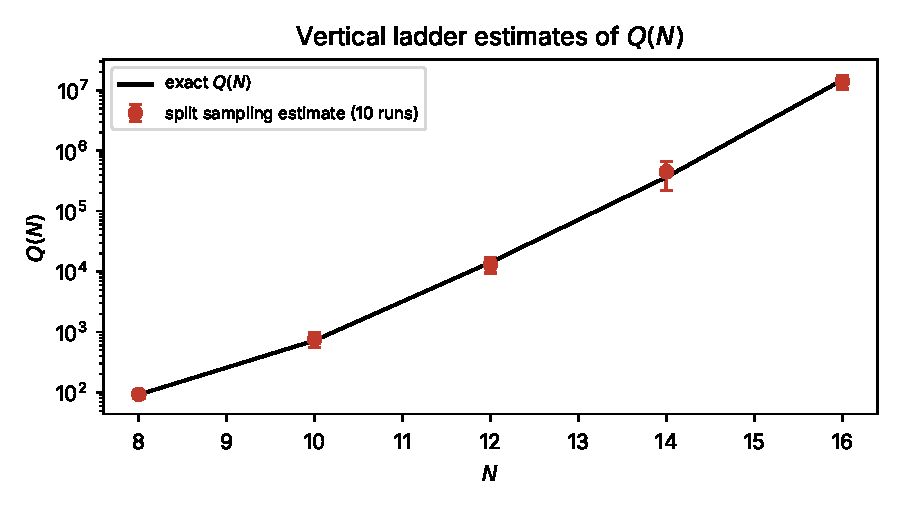
\includegraphics[width=0.9\textwidth]{fig_split.pdf}
\caption{Split sampling estimates of $Q(N)$ with one standard deviation error bars across ten runs, against the exact values.}
\label{fig:split}
\end{figure}

Table~\ref{tab:split} and Figure~\ref{fig:split} give the results. At every $N$ the mean estimate is within a factor $1.25$ of the exact count, and the exact count lies within $0.4$ standard deviations of the mean at every $N$. The coefficient of variation is between $0.13$ and $0.5$, and the ladder has between five and nine rungs. The total cost at $N = 16$ is $9 \times 400 \times 64 \approx 230\,000$ proposed swaps per run, against $16! \approx 2 \times 10^{13}$ permutations to enumerate.

Three observations. First, the number of rungs grows roughly like $N/2$, consistent with the mean energy $2N/3$ of Chapter~\ref{ch:phase} and the geometric decrease of each rung by a factor of about $0.3$ to $0.6$ at the upper rungs, and below $0.3$ over the last two to four rungs. Second, the last two rungs, from energy two to one and from one to zero, have the smallest ratios, and we expect, though we have not measured it per rung, that their level set chains are the slowest. Third, the relative error does not grow visibly with $N$ over this range, which is what one expects if the chain mixes in polynomial time on these level sets at these sizes. Whether it continues not to grow is the mixing conjecture of Chapter~\ref{ch:prp}, and the experiment cannot settle it; it can only say that for $N \le 16$ the walk works.

\section{The ladder}

The ladder from the last of the ten runs at each $N$ is in Table~\ref{tab:ladder}, which lists each level $m_t$ and the estimated ratio $\hat\theta_t = \hat Z_{m_t} / \hat Z_{m_{t-1}}$. Figure~\ref{fig:ladder} plots the cumulative $\log \hat Z_m$ against the level.

\begin{table}[t]
\centering
\small
\caption{The ladder of the last of the ten runs at each $N$: the level $m_t$ and the estimated ratio $\hat\theta_t$ at each rung, read from the top of the ladder down.}
\label{tab:ladder}
\begin{tabular}{rl}
\toprule
$N$ & $(m_t : \hat\theta_t)$ \\
\midrule
8 & $4{:}0.48, \; 3{:}0.54, \; 2{:}0.37, \; 1{:}0.26, \; 0{:}0.12$ \\
10 & $5{:}0.44, \; 4{:}0.63, \; 3{:}0.42, \; 2{:}0.30, \; 1{:}0.12, \; 0{:}0.04$ \\
12 & $6{:}0.39, \; 5{:}0.63, \; 4{:}0.48, \; 3{:}0.34, \; 2{:}0.19, \; 1{:}0.09, \; 0{:}0.04$ \\
14 & $7{:}0.36, \; 5{:}0.32, \; 4{:}0.40, \; 3{:}0.26, \; 2{:}0.16, \; 1{:}0.08, \; 0{:}0.04$ \\
16 & $9{:}0.39, \; 7{:}0.43, \; 6{:}0.48, \; 5{:}0.47, \; 4{:}0.30, \; 3{:}0.21, \; 2{:}0.15, \; 1{:}0.07, \; 0{:}0.01$ \\
\bottomrule
\end{tabular}
\end{table}

\begin{figure}[t]
\centering
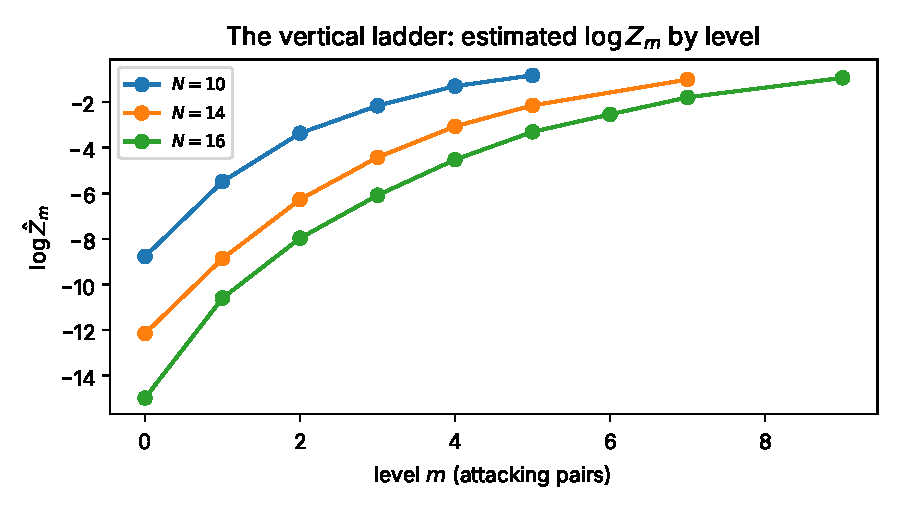
\includegraphics[width=0.9\textwidth]{fig_ladder.pdf}
\caption{Estimated $\log Z_m$ against the level $m$ for $N = 10$, $14$ and $16$, from one run each. The slope steepens as the level approaches zero.}
\label{fig:ladder}
\end{figure}

For $N = 8$ the exact ratios from Table~\ref{tab:dos} are $Z_4 / Z_5 = 0.71$, $Z_3 / Z_4 = 0.58$, $Z_2 / Z_3 = 0.36$, $Z_1 / Z_2 = 0.25$ and $Z_0 / Z_1 = 0.094$. The estimated ladder for $N = 8$ started at level four from the uniform population, where the exact $Z_4 = 0.46$, and its first estimated ratio $0.48$ matches; the subsequent ratios $0.54$, $0.37$, $0.26$ and $0.12$ are close to the exact $0.58$, $0.36$, $0.25$ and $0.094$, as one expects from a population of 400. The ladder is doing what the theory says it should.

The ratios at the bottom of the ladder decrease with $N$: the final ratio $\hat\theta_0 = \hat Z_0 / \hat Z_1$ is $0.12$ at $N = 8$, $0.04$ at $N = 10$ to $14$ and $0.01$ at $N = 16$. This is the steepening of the staircase in the low energy region, a geometric decrease whose limiting behaviour these data do not settle (Chapter~\ref{ch:experiments2} finds the fraction of time at energy zero consistent with decay like $1/N$). The ratio $N(0) / N(1)$ for $N = 8, 9$ from Table~\ref{tab:dos} is $0.104, 0.104$, and the estimated $\hat\theta_0$, which is $N(0) / (N(0) + N(1))$, keeps decreasing at larger $N$, with no limit visible. The final rung is the hardest in two senses at once: its ratio is the smallest, and we expect its chain, confined to permutations with at most one attacking pair, to be the slowest.

\section{Wang Landau and the density of states}

The Wang Landau\index{Wang Landau algorithm} algorithm of Appendix~\ref{app:alg} was run for $N = 10$ with the swap proposal, the flatness criterion that every visited level be visited at least $80\%$ of the mean, and the logarithm of the modification factor halved at each flat histogram. Figure~\ref{fig:wl10} compares the estimated density of states with the exact values from enumeration of the $3\,628\,800$ permutations.

\begin{figure}[t]
\centering
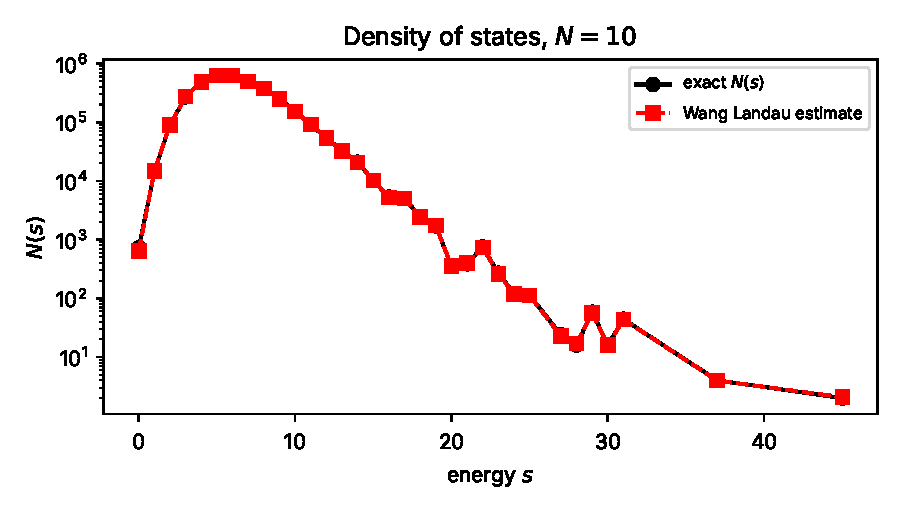
\includegraphics[width=0.9\textwidth]{fig_wl10.pdf}
\caption{Wang Landau estimate of the density of states for $N = 10$ against the exact enumeration, on a logarithmic scale. The estimate is accurate across the bulk and within $12\%$ at the ground state.}
\label{fig:wl10}
\end{figure}

The agreement is close across the bulk, with relative errors below $1\%$ for $s$ from $2$ to $7$ and $3\%$ at $s = 1$, and the ground state estimate is $642$ against the exact $724$, a relative error of $11\%$. The ground state is the hardest level for Wang Landau as it is for the ladder, and for the same reason: the chain reaches it rarely and the few visits give a noisy estimate of its weight. The flat histogram condition forces the chain to spend equal time at every level, which is the $1/N(s)$ reweighting of the multicanonical\index{multicanonical sampler} ensemble, and at the ground state the reweighting is by a factor of $10^3$ relative to the bulk; the chain achieves this by refusing almost every move out of a solution once it finds one, and it finds one rarely.

In the vertical coordinate Wang Landau is estimating all the step widths at once, by visiting them with equal frequency, where the ladder estimates them one at a time from the top. The ladder is more efficient for the ground state because it concentrates its effort there; Wang Landau is more informative because it returns the whole staircase. For counting one wants the ladder; for understanding the structure of the problem one wants Wang Landau, and the staircase it returns for $N = 10$ has 33 nonempty levels, of which the lowest, $s = 0$, carries all $724$ solutions and $0.02\%$ of the permutations.

\section{What the experiments show and do not show}

The experiments show that the vertical ladder is a working algorithm for the queens at the sizes where it can be checked, with a cost that is polynomial by design (a fixed $4N$ swaps per particle per rung) over the range $N \le 16$ and estimates that are unbiased to within sampling error. They show that the difficulty concentrates at the bottom rung, in the size of the ratio, as the theory predicts. And the mixing measurements of Chapter~\ref{ch:experiments2} (Table~\ref{tab:mixing}) suggest that the swap chain on low level sets is slow but not, at these sizes, stuck: the autocorrelation times are between $59$ and $430$ swaps for $N \le 16$.

They do not show that this continues. The mixing conjecture of Chapter~\ref{ch:prp} is about the limit $N \to \infty$, and no experiment at $N = 16$ can speak to it. What an experiment could do is estimate the mixing time\index{mixing time} of the bottom rung chain as a function of $N$ over a wider range, say $N = 8$ to $40$, by running it from many starting solutions and measuring the autocorrelation of some statistic, and look for the onset of exponential growth. We have not done this in this chapter; Chapter~\ref{ch:experiments2} does it for unconditioned boards. On unconditioned boards polynomial growth is what we expect, in line with the conjecture of Chapter~\ref{ch:swendsen}, and the place to look for an exponential is conditioned boards.
